\newpage
\section{Q3 --- Forecast Error vs. Predicted Hour}

\textbf{Research question:}

\begin{quote}
Is the forecast error dependent on the predicted hour? How does this relationship vary by weather variable, PJM zone, season, and year?
\end{quote}

\subsection{Data and Method}

Forecast errors were computed for the December 30 and December 31 forecast cycles and evaluated across the 48 forecast hours. To test whether forecast error depends on predicted hour, the Kruskal--Wallis test was applied across forecast-hour groups.

Because the dataset is very large, statistical significance alone is not the most useful measure of practical importance. Therefore, epsilon-squared effect size is emphasized more heavily than p-values when interpreting the strength of forecast-hour dependence.

\subsection{Descriptive Error Patterns by Forecast Hour and Weather Variable}

The per-variable forecast-hour line plots show how mean forecast error changes over the 48-hour horizon. The normalized all-variable heatmap provides a compact comparison across weather variables.

Overall, forecast-hour dependence is not uniform across variables. GHI and pressure show clearer forecast-hour structure, while wind direction and wind-component errors show weaker forecast-hour structure.


\subsection{Statistical Evidence for Forecast-Hour Dependence}

The all-site Kruskal--Wallis epsilon-squared summary provides the main statistical evidence for whether forecast error depends on forecast hour.

The strongest forecast-hour dependence appears for GHI and pressure, with mean epsilon-squared values of 0.0524 and 0.0506, respectively. Relative humidity and temperature show moderate forecast-hour dependence, with mean epsilon-squared values of 0.0308 and 0.0284. Wind speed has a mean epsilon-squared value of 0.0149, U wind, V wind, and wind direction have the weakest dependence with the values of 0.0087, 0.0085, and 0.0044 respectively.

These results suggest that forecast hour matters most for GHI and pressure errors, moderately for relative humidity and temperature errors, and weakly for wind-variable errors.

\begin{figure}[H]
    \centering
    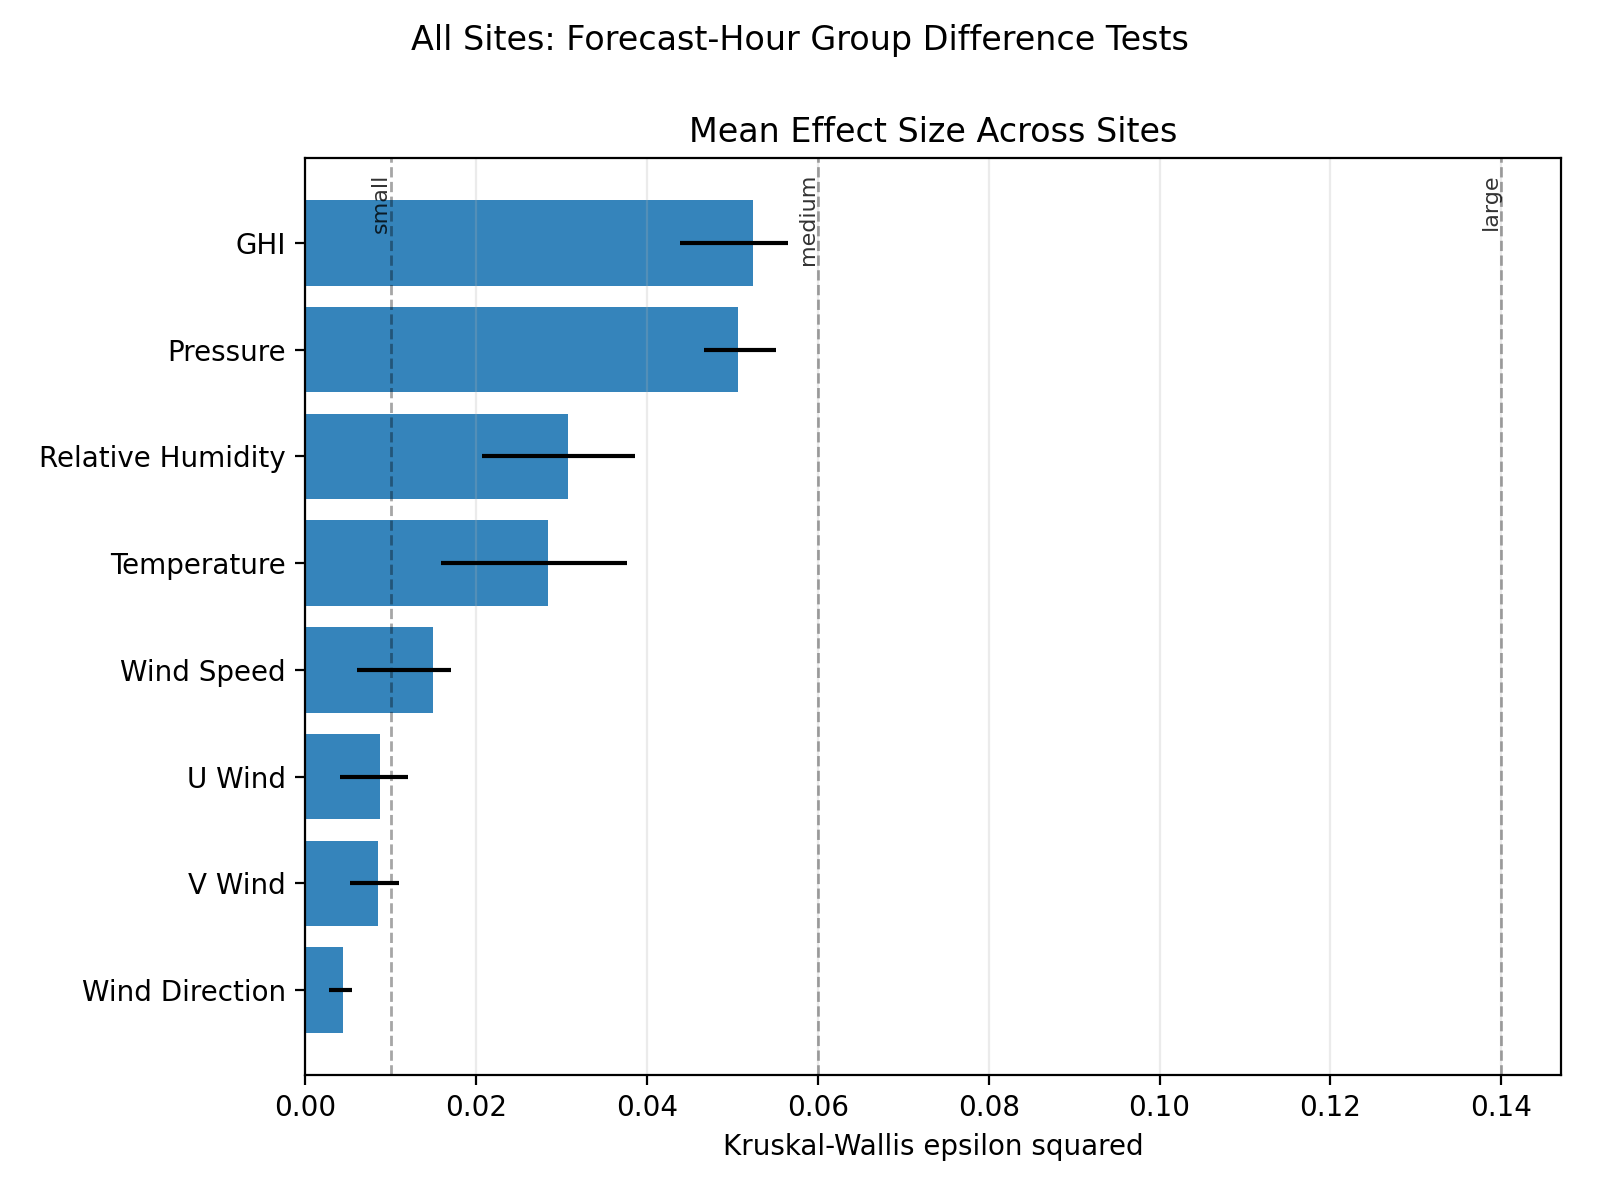
\includegraphics[width=0.60\textwidth]{figures/Q3/section_5_figures/5_2_statistical_test/kruskal_forecast_hour_epsilon_summary_allsites.png}
    \caption{Mean epsilon-squared effect size from Kruskal--Wallis tests across forecast-hour groups.}
    \label{fig:kruskal_forecast_hour_summary}
\end{figure}

\subsection{Variation by Season}

The forecast-hour-by-season heatmap and summary figure show whether the forecast-hour relationship changes by season.

Pooled across seasons, pressure, GHI, relative humidity, and temperature have the largest forecast-hour effect sizes. Summer is especially important for relative humidity, temperature, and pressure. Fall also shows strong pressure forecast-hour dependence. Wind variables remain weaker than radiation, pressure, temperature, and humidity, although summer increases wind-speed and wind-component effects somewhat.

\begin{figure}[H]
    \centering
    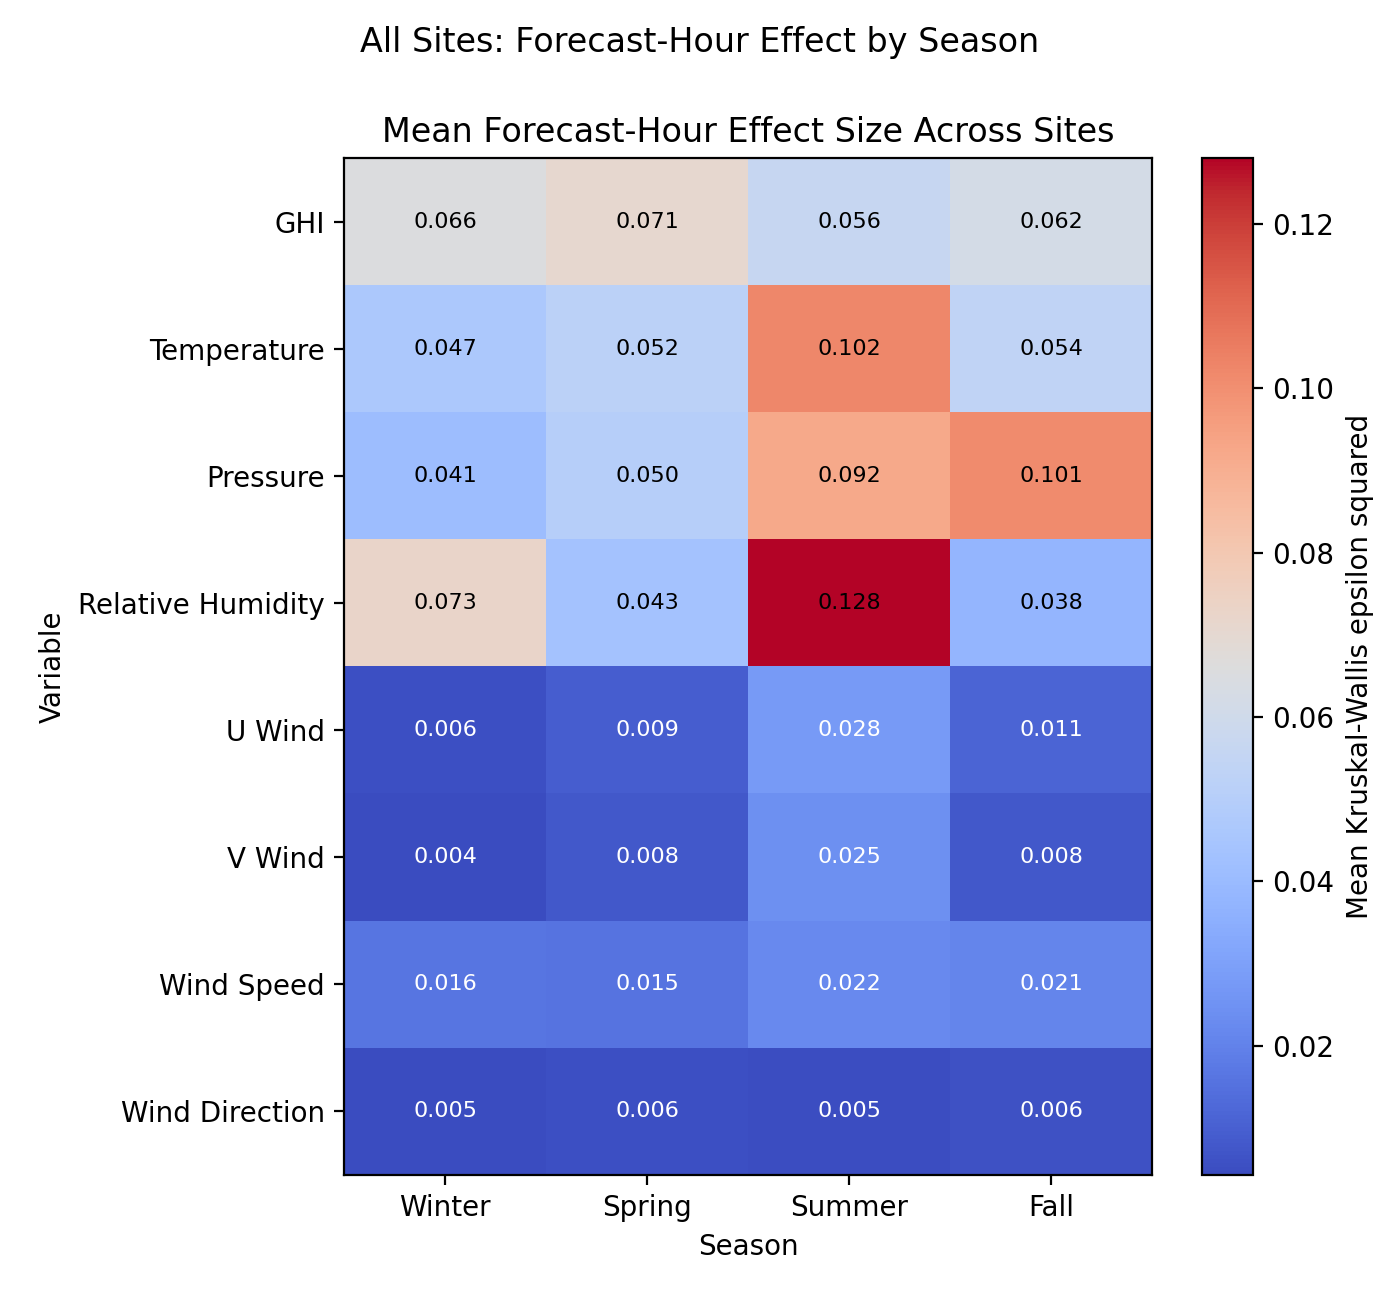
\includegraphics[width=0.60\textwidth]{figures/Q3/section_5_figures/5_3_season/kruskal_forecast_hour_by_season_epsilon_heatmap_allsites.png}
    \caption{Forecast-hour dependence by season, measured using epsilon-squared effect size.}
    \label{fig:forecast_hour_season_heatmap}
\end{figure}

\begin{figure}[H]
    \centering
    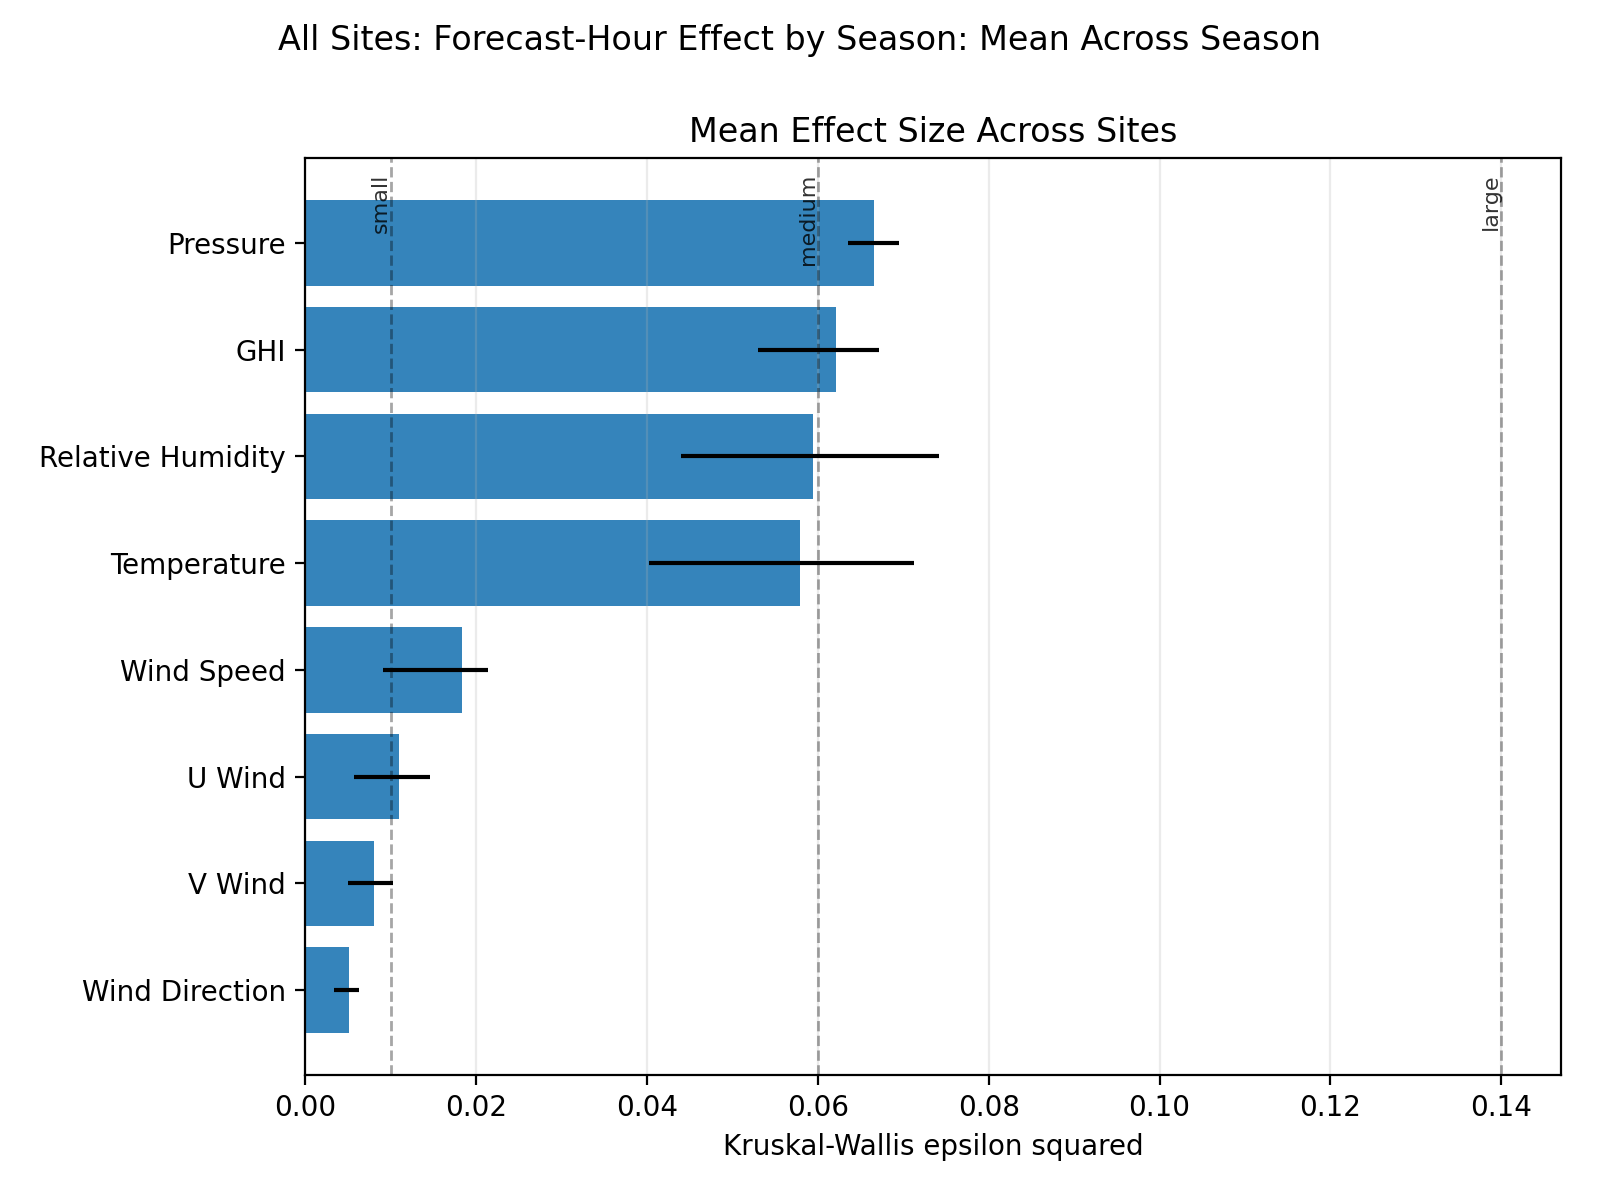
\includegraphics[width=0.60\textwidth]{figures/Q3/section_5_figures/5_3_season/kruskal_forecast_hour_by_season_epsilon_summary_allsites.png}
    \caption{Seasonal summary of forecast-hour dependence across weather variables.}
    \label{fig:forecast_hour_season_summary}
\end{figure}

\subsection{Variation by Year}

The forecast-hour-by-year heatmap and summary figure show whether forecast-hour dependence changes across years.

The year-stratified pattern is broadly stable. Pressure and GHI remain the strongest forecast-hour-dependent variables in 2022, 2023, and 2024. Temperature and relative humidity are consistently moderate. Wind speed, U wind, V wind, and wind direction remain comparatively weak.

\begin{figure}[H]
    \centering
    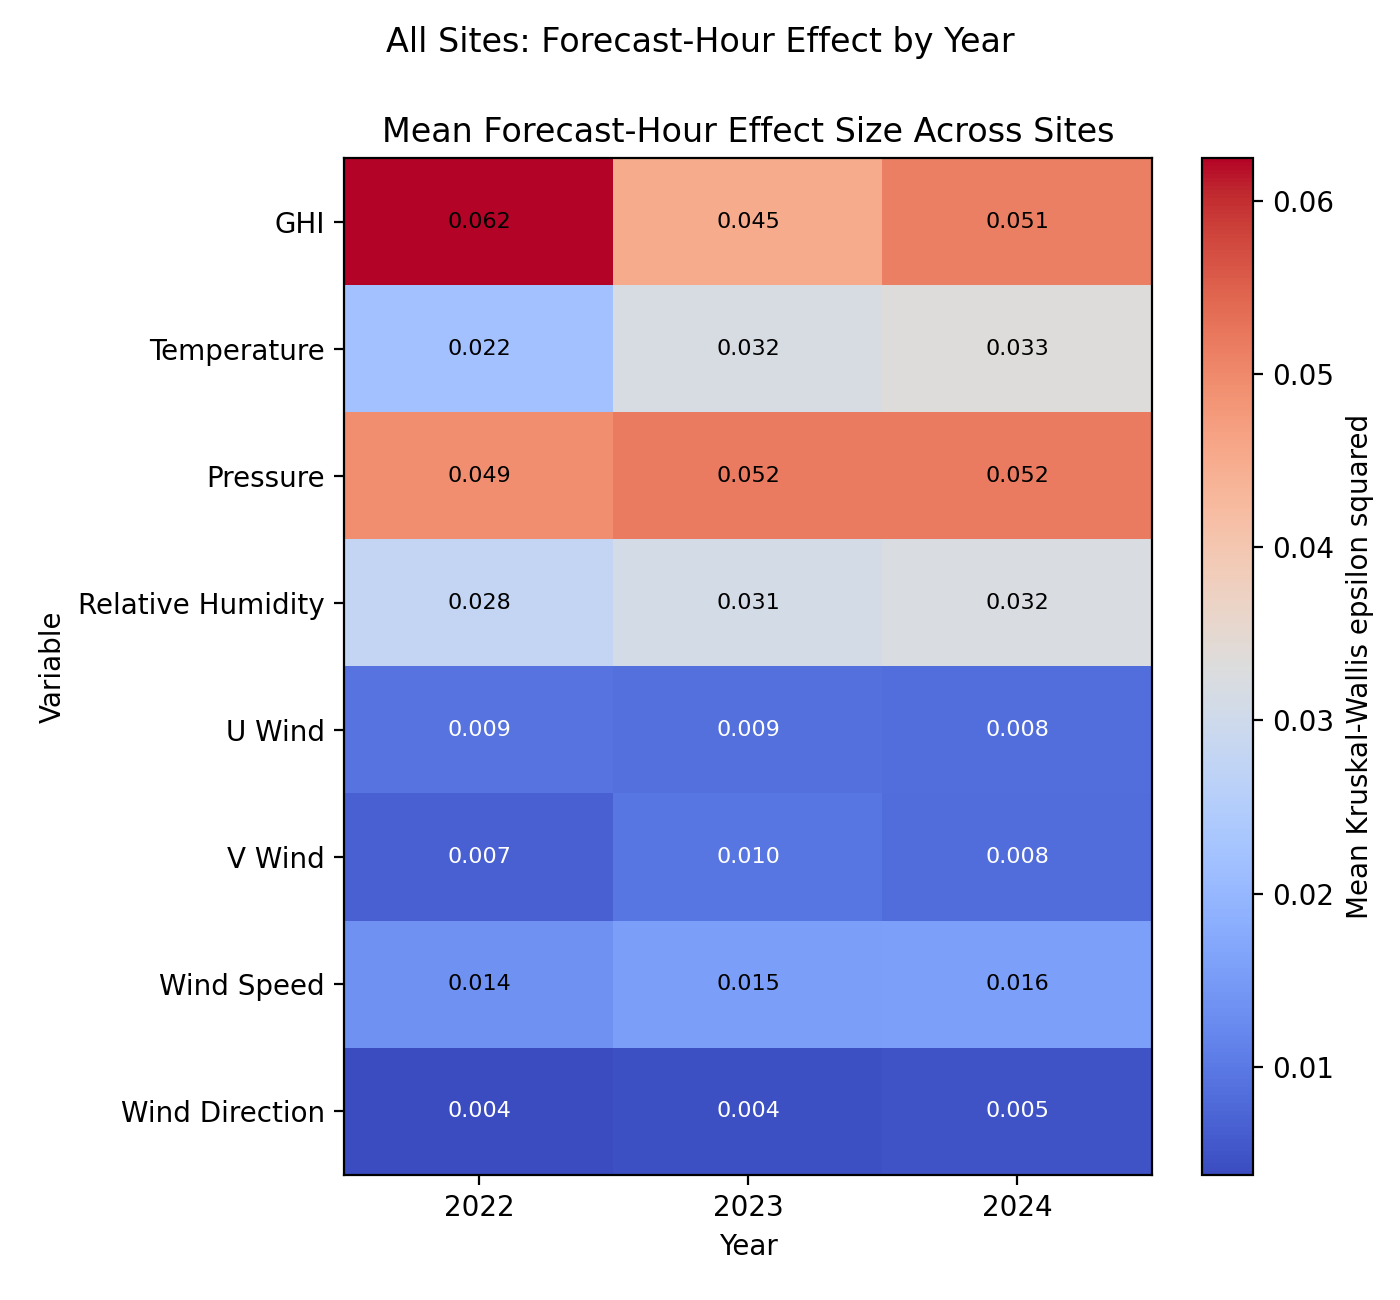
\includegraphics[width=0.60\textwidth]{figures/Q3/section_5_figures/5_4_year/kruskal_forecast_hour_by_year_epsilon_heatmap_allsites.png}
    \caption{Forecast-hour dependence by year, measured using epsilon-squared effect size.}
    \label{fig:forecast_hour_year_heatmap}
\end{figure}

\begin{figure}[H]
    \centering
    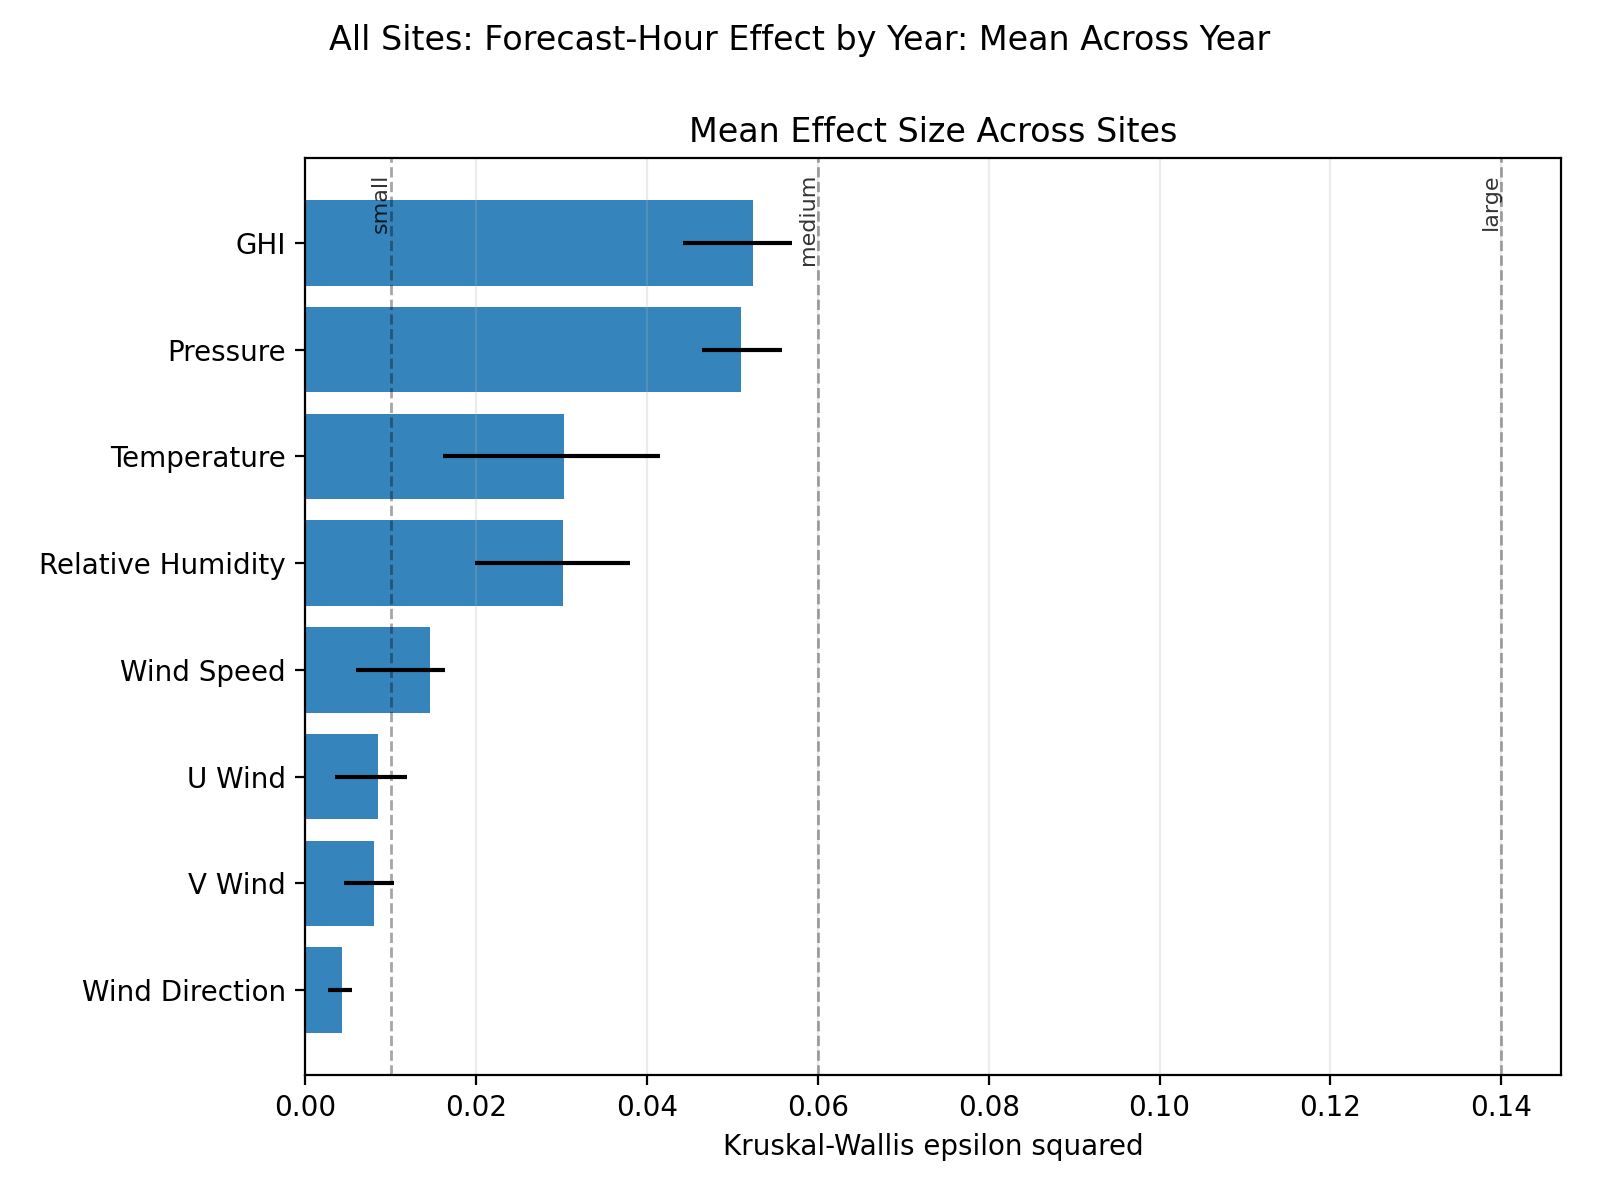
\includegraphics[width=0.60\textwidth]{figures/Q3/section_5_figures/5_4_year/kruskal_forecast_hour_by_year_epsilon_summary_allsites.png}
    \caption{Yearly summary of forecast-hour dependence across weather variables.}
    \label{fig:forecast_hour_year_summary}
\end{figure}

\subsection{Conclusion}

Forecast error is dependent on forecast hour, but the strength of that dependence varies substantially by weather variable. The clearest forecast-hour effects occur for GHI and pressure, followed by relative humidity and temperature. Wind variables show weaker dependence on forecast hour.

Seasonal stratification reveals stronger forecast-hour effects in specific seasons, especially summer for temperature and relative humidity and fall or summer for pressure. Year-to-year differences are smaller than variable and seasonal differences. PJM-zone variation still requires a dedicated zone-stratified analysis.
